\documentclass[18pt]{article}

\usepackage[utf8]{inputenc}
\usepackage[T1]{fontenc}
\usepackage{ragged2e}
\usepackage{caladea}
\usepackage{graphicx}
\usepackage{longtable}
\usepackage{wrapfig}
\usepackage{rotating}
\usepackage{epigraph}
\usepackage[normalem]{ulem}
\usepackage{hyperref}
\usepackage{amsmath}
\usepackage{amssymb}
\usepackage{capt-of}
\usepackage{fancyhdr}

\title{
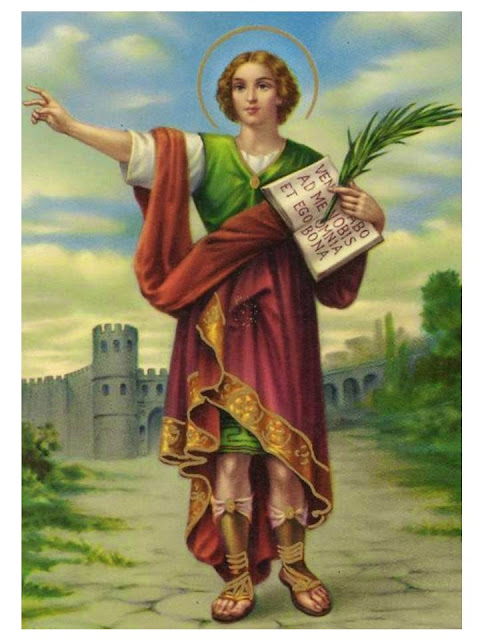
\includegraphics[scale=.55, trim={10cm, 0, 10cm, 0}]{./assets/imagem.jpg}
\par
Novena a São Pancrácio
}

\date{Data de Início: 03/05 \quad Data Litúrgica: 12/05}

\renewcommand{\contentsname}{Sumário}

\begin{document}

\thispagestyle{empty}

\maketitle

\begin{center}
Visite-nos no Telegram: \url{https://t.me/CotidieNovena}
\end{center}

\pagestyle{fancy}
\fancyhf{}
\fancyfoot[LO, CE]{

\includegraphics[scale=0.2]{./assets/cross.png} São Pancrácio, rogai por nós!
}
\fancyfoot[R]{\thepage}

\newpage

\tableofcontents

\newpage

%%%%%%%%%%%%%%%%%%%%%%%%%%%%%%%%%%%%% História %%%%%%%%%%%%%%%%%%%%%%%%%%%%%%%%%%%%%%%%%%%

\begin{justify}
\begin{center}
\section{História}\label{sec:História}
\end{center}

São Pancrácio nasceu por volta do ano 289, na Frígia (atual Turquia). Órfão desde cedo, mudou-se para Roma com seu tio Dionísio, onde ambos se converteram ao cristianismo. Durante as perseguições do imperador Diocleciano, Pancrácio, ainda adolescente, recusou-se a renunciar à fé em Cristo. Por sua coragem e fidelidade, foi martirizado por decapitação, provavelmente no ano 304, quando tinha apenas 14 anos.

A devoção a São Pancrácio se espalhou rapidamente por toda a Igreja, especialmente como intercessor dos jovens, dos trabalhadores e dos que buscam emprego. É considerado também protetor contra falsas testemunhas e juramentos injustos. Sua festa litúrgica é celebrada em 12 de maio.

\vfill

\begin{center}
\href{https://www.a12.com/santuario/noticias/sao-pancracio-o-santo-dos-empregados-e-dos-necessitados}{Fonte: Santuário Nacional Aparecida}
\end{center}
\end{justify}

%%%%%%%%%%%%%%%%%%%%%%%%%%%%%%%%%%%%% Orações %%%%%%%%%%%%%%%%%%%%%%%%%%%%%%%%%%%%%%%%%%%

\newpage

\begin{center}
\section{Orações}\label{sec:Orações}
\textit{Em nome do Pai, e do Filho, e do Espírito Santo. Amém.}
\end{center}

\subsection*{Oração Inicial}
Ó glorioso São Pancrácio, vós que, ainda jovem, destes testemunho de fé e coragem diante das perseguições, alcançai-me a graça de amar a Deus sobre todas as coisas, de perseverar na fé e de ser fiel em todas as situações da minha vida. Intercedei por mim junto ao Senhor, para que eu obtenha as graças de que tanto preciso, especialmente (mencionar a intenção). Amém.

\subsection*{Oração à Santíssima Virgem}
Reconheço-vos e venero-Vos, ó Virgem Santíssima, Rainha dos Céus, Senhora e Patrona do Universo, como a Filha do Eterno Pai, Mãe de Seu diletíssimo Filho, e Esposa amantíssima do Espírito Santo; e, prostrado aos pés de Vossa grande Majestade, com a maior humildade Vos suplico, por aquela divina caridade de que fostes sumamente cheia em Vossa Assunção ao Céu, que me obtenhais a singular graça e misericórdia de me pôr sob Vossa seguríssima e fidelíssima proteção e de me receber no número daqueles felicíssimos e afortunados servos que levais escritos em Vosso virginal peito.

Dignai-vos, ó Mãe e Senhora minha clementíssima, aceitar meu miserável coração, minha memória, minha vontade e as demais potências e sentidos meus interiores e exteriores. Aceitai meus olhos, meus ouvidos, minha boca, minhas mãos e meus pés, regei-os conforme o beneplácito de Vosso Filho, a fim de que com todos os meus movimentos tenha a intenção de Vos tributar glória infinita. E por aquela sabedoria com que vos iluminou Vosso amantíssimo Filho, Vos rogo e suplico me alcanceis luz e claridade para conhecer-me bem a mim mesmo, meu nada, e particularmente meus pecados, para odiá-los e detestá-los sempre. Alcançai-me a luz para conhecer as tentações do inimigo infernal e seus combates ocultos e manifestos.

Especialmente, piedosíssima Mãe minha, vos suplico a(s) graça(s) seguinte(s): (mencionar graça desejada).

\subsection*{Oração à Santíssima Trindade (para o final de todos os dias)}

\textbf{Adoração ao Pai Eterno}

Pai-Nosso, uma Ave-Maria e um Glória.

Adoro-vos, Oh! Pai eterno, com toda a Corte Celestial, meu Deus e Senhor, e Vos dou infinitas graças em nome da Santíssima Virgem, Vossa Filha muito amada, por todos os dons e privilégios com que a adornastes, especialmente por aquele poder com que A enaltecestes em Sua gloriosa Assunção aos Céus.

\textbf{Adoração ao Eterno Filho}

Pai-Nosso, Ave-Maria e Glória.

Adoro-vos, Oh! Eterno Filho, com toda a Corte Celestial, meu Deus, Senhor e Redentor, e Vos rendo graças infinitas em nome da Santíssima Virgem, Vossa muito amada Mãe, por todos os dons e privilégios com que a adornastes, especialmente por aquela suma sabedoria com que A ilustrastes em Sua gloriosa Assunção ao Céu.

\textbf{Adoração ao Espírito Santo}

Pai-Nosso, Ave-Maria e Glória.

Adoro-vos, Espírito Santo Paráclito, por meu Deus e Senhor, e Vos dou infinitas graças com toda a Corte Celestial, em nome da Santíssima Virgem, Vossa amantíssima Esposa, por todos os dons e privilégios com que a adornastes, especialmente por aquela perfeitíssima e divina caridade com que inflamastes Seu Santíssimo e Puríssimo Coração no ato de Sua gloriosíssima Assunção ao Céu; e humildemente Vos suplico em nome de Vossa Imaculada Esposa, me outorgueis a graça de me perdoar todos os gravíssimos pecados que tenho cometido desde o primeiro instante em que pude pecar, até o presente, os quais me doem infinitamente: faço firme propósito de morrer antes de voltar outra vez a ofender a Vossa divina Majestade; e pelos altíssimos méritos e eficacíssima proteção de Vossa amantíssima Esposa, Vos suplico me concedais o preciosíssimo dom de Vossa graça e divino amor, dando me aquelas luzes e particulares auxílios com os quais Vossa eterna Providência tinha determinado salvar-me, e conduzir-me a Vós.

\textbf{Em nome do Pai, e do Filho, e do Espírito Santo. Amém.}

\vfill

%%%%%%%%%%%%%%%%%%%%%%%%%%%%%%%%%%%%% Orações de Cada Dia %%%%%%%%%%%%%%%%%%%%%%%%%%%%%%%%%%%%%%%%%%%

\newpage

\section*{Orações de Cada Dia}

\subsection*{Primeiro Dia}
Nosso coração foi criado para amar: o que mais tens que amar é a Deus; mais que a todas as pessoas, mais que a todas as riquezas do mundo, e desta maneira evitarás também muitos desenganos. Desta maneira o fez São Pancrácio, e por isso alcançou tantos favores de Deus. Peça-lhe de coração esta graça; viverás mais tranquilo e alcançarás sua proteção em tudo o que necessites.

\textit{Concluir com as orações à Santíssima Trindade.}

\subsection*{Segundo Dia}
Deus permite que amemos a nossa família e a outras pessoas, enquanto não seja obstáculo para amar a Deus. Assim o fazia o glorioso São Pancrácio, e desta maneira encaminhou muitas almas ao Céu. Peça-lhe de todo coração que ames como bons irmãos às outras pessoas, a fim de que amemos mais a Deus e obtenhamos muitas graças do glorioso São Pancrácio.

\textit{Concluir com as orações à Santíssima Trindade.}

\subsection*{Terceiro Dia}
São Pancrácio tinha um coração tão bom que sempre se compadecia dos pobres e desgraçados: por isso, conseguiu tantas graças do Céu; procura você também imitá-lo nestas virtudes, e assim lograrás por sua intercessão obter muitas graças de Deus.

\textit{Concluir com as orações à Santíssima Trindade.}

\subsection*{Quarto Dia}
O glorioso São Pancrácio não somente procurou ser bom, senão que trabalhava para poder guiar outras almas ao Céu, e por isso Deus lhe concedeu tanto poder em favor de seus devotos. Procura você também fazer que possa propagar essa devoção e procurar que outros vão pelo caminho do Céu. Assim conseguirás muitas graças, especialmente as que tem necessidade agora que fazes esta novena.

\textit{Concluir com as orações à Santíssima Trindade.}

\subsection*{Quinto Dia}
No mundo, há muitas pessoas que, por respeitos humanos, não são boas, para que não as tenhamos como fanáticas. Procura que não sejas você um desses: senão que, à imitação de São Pancrácio, sempre defendas a verdade e as coisas boas. Desta maneira, conseguirá tudo de que necessites, por intercessão de São Pancrácio, que atenderá sempre a seus rogos.

\textit{Concluir com as orações à Santíssima Trindade.}

\subsection*{Sexto Dia}
Uma das coisas que custa mais a nosso coração é perdoar aos que nos têm agravado. Peça ao glorioso São Pancrácio que lhe alcance esta graça quando alguém lhe agrave (ofenda), já que ele perdoou até aos que o martirizaram, e não duvide de que estarás depois mais tranquilo e conseguirá para você para sua família mais do que possa esperar.

\textit{Concluir com as orações à Santíssima Trindade.}

\subsection*{Sétimo Dia}
Neste mundo se tem de ter muita paciência em tudo, pois vem mais contrariedades do que esperamos. Toma por modelo ao glorioso São Pancrácio, que em tudo se conformava com a vontade de Deus, e assim logrou viver tranquilo e ser um grande Santo, em meio de muitas penas. Peça-lhe de bom coração que o ajude e lhe concederá esta graça e muitas mais.

\textit{Concluir com as orações à Santíssima Trindade.}

\subsection*{Oitavo Dia}
Assim como você quer o retrato de seus pais e outras pessoas amigas, também convém que queiras a imagem do glorioso São Pancrácio, não duvidando que desde o Céu ele vê como se ajoelha ante o altar em que está colocado. Quanto com maior fervor você o faça, mais ele rogará a Deus para que lhe conceda o que lhe pedes nesta novena, tanto para você, como para as pessoas de vossa família.

\textit{Concluir com as orações à Santíssima Trindade.}

\subsection*{Nono Dia}
Agora que terminas a novena, estás animado e tens mais desejos de amar a São Pancrácio, e portanto, de se fazer digno de que possa ir ao Céu para fazer-lhe companhia. Não duvide que ali o espera, e irá!, se cumprir bem suas obrigações vivendo como um bom cristão; conseguindo já, desde agora, sua proteção em tudo, tanto para ti, como para vossa família.

\textit{Concluir com as orações à Santíssima Trindade.}

\vfill

\subsection*{Créditos:}

\href{https://precantur.blogspot.com/2015/05/novena-sao-pancracio.html}{Fonte: Precantur - Blog}

\end{document}
